\chapter{\ac{ser} Development}
\label{chapter:strat}

\section{Datasets}

In this section, we will detail the two utilized datasets that were used for the development of our \ac{ser} system.
By utilizing two distinct datasets for our analysis, we are able to make the models more robust and effective, making the results less prone to overfitting.

The first dataset was used as a development set, which we used to explore and select the best features for the traditional approach models.

The second dataset was used as a training and test set for evaluating the performance of our predictive models and determining the most effective strategies.

\subsection{eNTERFACE'05}

The eNTERFACE’05 emotion database \cite{Martin2006} was designed and collected during the eNTERFACE’05 workshop in \citeyear{Martin2006}. The dataset contains audio and visual data from 42 subjects, coming from 14 different nationalities. Among the subjects, a percentage of 35 are men, while the remaining 7 are women, and, all the experiments were driven in English.

\begin{table}[H]
	\centering
	\caption{eNTERFACE'05 subjects nationalities}
	\label{tab:enterfaceDiversity}
	\begin{tabular}{lc|lc}
		\toprule
		Country &Number of Subjects &Country &Number of Subjects\\
		\midrule
		Belgium & 9 & Cuba     & 1\\
		Turkey  & 7 & Slovakia & 1\\
		France  & 7 & Brazil   & 1\\
		Spain   & 6 & U.S.A.   & 1\\
		Greece  & 4 & Croatia  & 1\\
		Italy   & 1 & Canada   & 1\\
		Austria & 1 & Russia   & 1\\
		\bottomrule
	\end{tabular}
\end{table}


This dataset contains six discrete annotated emotions: \begin{enumerate*}\item anger \item fear \item surprise \item happiness \item sadness \item disgust. \end{enumerate*} Each subject was asked to listen to six successive short stories, each eliciting a particular emotion. If two human experts judged the reaction expressing the emotion unambiguously, then the sample was added to the database. Afterward, they were recorded saying five different sentences for each emotion, and, in total, there are 212 video and audio sequences per annotated emotion, recorded with a sample rate of 16000 Hertz.

The selection of this dataset for feature analysis and selection was based on several factors. Firstly, the controlled environment of the dataset ensured that the data was collected under controlled conditions, which minimized the impact of external factors that could have influenced our analysis. Moreover, the diversity of the subjects included in this dataset made it possible to identify and select features that are representative of several groups of people.

Another key factor in choosing this data was its size. Due to the limited size of this dataset, we are able to utilize computationally expensive methods, such as feature selection algorithms, that would have been prohibitively expensive with larger datasets.

Finally, the elicited nature of the data in this dataset was considered an essential aspect of our selection process. Elicited obtained data tends to be more genuine than acted, therefore, it provides a more accurate representation of video conferences' natural contexts.

\subsection{\ac{iemo}}

The \ac{iemo} database \cite{Busso2008}, created in \citeyear{Busso2008}, is an acted and elicited multimodal and multi-speaker database. It consists of 12 hours of audiovisual data, including video, speech, motion capture of face, and text transcriptions.

Sessions were manually segmented into utterances, spoken by 10 (5 female and 5 male) professional actors in fluent English. Each utterance was annotated by at least 3 human annotators in 9 categorical attributes, and, in addition, it was annotated with 3-dimensional attributes using the \ac{vad} emotion model. Similar to the development dataset, this data was collected using emotion elicitation techniques such as improvisations and scripts. Figure \ref{fig:bar_plots_distribution} from the research article \ref{Busso2008}, demonstrates that there is a similar amount of annotated labels on scripted and spontaneous sessions on this dataset.

\begin{figure}[H]
	\centering
	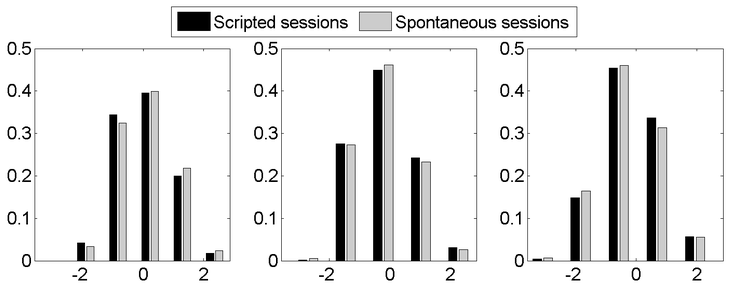
\includegraphics[width=.8\linewidth]{figs/4_1_traditional/scripted_spont_distribution.png}
	\caption{Distribution of the emotional content of the IEMOCAP corpus in terms of (a) valence, (b) activation, and (c) dominance. The results are separately displayed for scripted (black) and spontaneous (gray) sessions.}
	\label{fig:bar_plots_distribution}
\end{figure}

Several researchers when utilizing the IEMOCAP dataset tend to only perform 4 class sentiment analysis, and also, consider the emotion of excitement as happiness to even out the distribution of files per emotion, as shown in the table \ref{tab:dataDist}, ending up with a total of 5531 audio files, recorded with a sample rate of 16000 Hertz.

\begin{table}[H]
	\centering
	\caption{Number of Audio Files Used per Emotion from the IEMOCAP dataset.}
	\label{tab:dataDist}
	\begin{tabular}{cc}
		\toprule
		Emotion & Number of Audio Files \\
		\midrule
		Anger & 1103\\
		Happiness &  1636\\
		Neutral &  1708\\
		Sadness & 1084\\
		\bottomrule
	\end{tabular}
\end{table}


Overall, this second dataset is a well-suited resource for our study, as the multimodal data, annotated using both discrete and dimensional models, allows us to perform a wide range of investigations, researchers have also noted the high quality of this dataset, being frequently used in the literature for evaluating emotion recognition models. This enables us to make well-founded comparisons of our own developed models, which is why we utilized \ac{iemo} as a training and testing dataset for our \ac{ser} models and to explore strategies and biases by stratifying the data.
